%% This is the main content about this article. I should list them in an order
%% How to balance the existing model, positive and negative instance together, I shall use the dfg-method to create a dfg-matrix to incorporate the impact.
%% how to introduce them into adding long-term dependency feature. After mining the model by Inductive Miner, we have a model without long-term dependency, but we need to change the model and give the right examples.. 
%% If we change the data set, then we need to change the model into another parts, but the current methods can not solve it..
%% Should we also separate them into different sections?? Yes, we need it
%% Also, to delete the silent transition, as one option feature in our methods, we only delete it, in this situation, which will not affect the model behavoirs.

%% Or we could organize the content in this way:
%%  -- put the whole structure ahead and put all that we want to talk
%%  -- list the steps 
%%    ++ dfg-method to balance the directly-follows relation and create the corresponding directly-follows graph
%%    ++ add long-term dependency on the model
%%    ++ delete the silent transitions on the model as a post model

%% Put some words here
This chapter describes our repair algorithm to incorporate the negative instances on process enhancement. In the beginning, the architecture of this algorithm is provided to give an overview. Details of main steps are represented in the following order. Firstly, the impact of the existing model, positive and negative instances are balanced in the media of the directly-follow relations. Inductive Miner is then applied to mine process models from those directly-follows relations. Next, we detect and add long-term dependency on the generated process models. Furthermore, the model in Petri net with long-term dependency is  post-processed for the sake of simplicity. 
\section{Architecture}
%% Describe the 
Figure \ref{fig:architecture} shows the steps of our strategy to enhance a process model. The basic inputs are an event log, and a Petri net. The traces in event log have an attribute for the classification labels of positive or negative in respect to some KPIs of business processes. The Petri net is the referenced model for the business process. To repair model with negative instances,  those steps are conducted.
\begin{figure}
	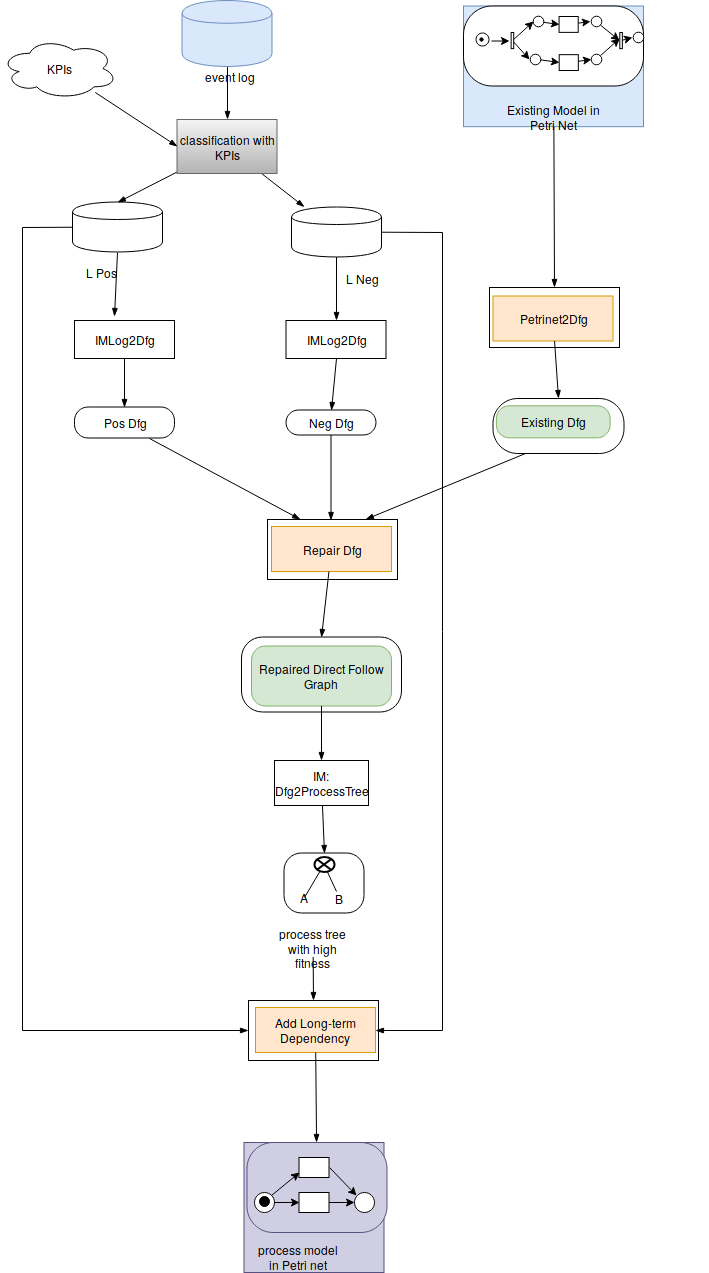
\includegraphics[width=0.9\textwidth, height=0.9\textheight]{figures/algorithm/FD_architecture_detail_02.png}
	\caption[Model Repair Architecture]{Model Repair Architecture -- \small Rectangles represents processes and output data in eclipse shape, especially customized processes and data are in doubled lattice shape. Input event log and existing model are in blue, KPIs are in cloud. The final output is a Petri net in purple. }
	\label{fig:architecture}
\end{figure} 
\begin{itemize}
	\item \emph{Generate directly-follows graphs}\quad 
	Three directly-follows graphs are generated respectively for the existing model, positive instance and negative instances from the event log.
	\item \emph{Repair directly-follows graph} \quad
	The three directly-follows graphs are combined into one single directly-follows graph after balancing their impact.
	\item \emph{Mine models from directly-follows graph} \quad
	Process models are mined from the repaired directly-follows graph by Inductive Miner as intermediate results.
	\item \emph{Add long-term dependency} \quad
	Long-term dependency is detected on the intermediate models and finally added on the Petri net. To simplify the model, the reduction of silent transitions can be applied at the end.
\end{itemize}
More details can be provided in the following sections.

\section{Generate directly-follows graph}
Originally, the even log $L$ is split into two sublogs, called $L_{pos}$ and $L_{neg}$. $L_{pos}$ contains the traces which are labeled as positive, while $L_{neg}$ contains the negative instances in the event log. Then, those two sublogs are passed to an existing procedure \emph{IMLog2Dfg} from \cite{leemans2013discovering}. \emph{IMLog2Dfg} traverses traces in the event log, extracts directly-follows relations of activities, and generates a directly-follows graph based on those relations. By using \emph{IMLog2Dfg}, $G(L_{pos})$ and $G(L_{neg})$ are generated respectively from positive and negative instances.
% Actually we can simplify those steps and reduce the time, but here just keep it like this.

To generate a directly-follows graph from a Petri net, we gather the model behaviors by building a transition system. A transition system for a Petri net is composed of \emph{states} and \emph{transitions}. \emph{States} are the possible markings of this Petri net. \emph{Transitions} are activities from event log. Those transitions connect states as an arc from its enable marking to the marking after its execution. For each state, transitions pointed from this state are directly followed by transitions pointed to this state. By checking the transition system. directly-follows relations for the models are extracted. Based on those relations, we create a directly-follows graph for the existing model.

From the positive and negative event logs, we can get the cardinality for corresponding directly-follows graph to represent the strength of this directly-follows relation. However, when the existing model is transformed into  directly-follows graph $G(L_{ext})$, there is no point to assign cardinality on each edge. So we just set cardinality with 1 for each arc. 
\section{Repair directly-follows graph}
%% we can have subsection on it. How to repair on them??? 
To combine all information of the directly-follows graphs from the positive , negative instances and the existing model, namely $G(L_{pos})$, $G(L_{neg})$ and $G(L_{ext})$, the cardinality in directly-follows graphs is unified as the percentage to the sum of total cardinalities with a range [0-1].
% here we already changed the definitions for the unifications..now it became as the percentage of the cardinality to its whole cardinality. No matter negative or positive ones...we can do it, right? 
\begin{definition}[Unified cardinality]
Given a directly-follows graphs $G(L)$ for a model, the unified cardinality of each directly-follows relation is defined as \[ U(E(A,B)) = \frac{Cardinality(E(A,B))}{Cardinality(E(*,*))}, with \]
	\[ Cardinality(E(*,*))=\sum{Cardinality(E(X,Y) \vert E(X,Y) \in G(L))}  \] 
	for start activities A, 
	\[ U(Start(A)) = \frac{Cardinality(Start(A))}{Cardinality(Start(*))} \]
	Similarly for end activities B,
	\[ U(End(B)) = \frac{Cardinality(End(B))}{Cardinality(End(*))} \]
$E(*,*)$ means all edges in the directly-follows graph, $E(*,B)$ means all edges with target B, $Start(*)$ represents all start nodes, and $End(*)$ represents all end nodes. 
\end{definition}

After the unification, the impact from existing model, positive and negative instances is in the same level and is balanced by subtracting the negative unification from the sum of existing and positive unification. The output from this balance is as the generated unification for the repaired model. 
\begin{definition}[Unified cardinality for directly-follows graph $G_{new}$]
The unified cardinality for the repaired directly-follows relations is defined in the following.
	\begin{itemize}
		\item For one directly-follows relation, \[ U(E_{G_{new}}(A,B)) =  U(E_{G_{ext}}(A,B))+ U(E_{G_{pos}}(A,B))  - U(E_{G_{neg}}(A,B)) \] 
		
		if $U(E_{G_{new}}(A,B)) > 1 , U(E_{G_{new}}(A,B)) =1$, \\
		if $U(E_{G_{new}}(A,B)) < 0 , U(E_{G_{new}}(A,B)) =0$; 
	    
		\item For start acivities A, we have 
		\[ U(Start_{G_{new}}(A)) =  U(Start_{G_{ext}}(A)) + U(Start_{G_{pos}}(A)) - U(Start_{G_{neg}}(A)) \]
		
		if $U(Start_{G_{new}}(A)) > 1 , U(Start_{G_{new}}(A)) =1$, \\
		if $U(Start_{G_{new}}(A)) < 0 , U(Start_{G_{new}}(A)) =0$;  
		
		\item For end activities B, we have
		\[ U(End_{G_{new}}(A)) = U(End_{G_{ext}}(A)) +  U(End_{G_{pos}}(A)) - U(End_{G_{neg}}(A)) \]
		if $U(End_{G_{new}}(A)) > 1 , U(End_{G_{new}}(A)) =1$, \\
		if $U(End_{G_{new}}(A)) < 0 , U(End_{G_{new}}(A)) =0$. 
	\end{itemize}
\end{definition} 
%% Here we add the control weight on it
In the real life, there exists various needs to address the impact either from the existing model, the positive instances or the negative instances. To meet this requirement, three control parameters in range [0-1] are assigned respectively to each unified cardinality from the existing model, and positive and negative instances. The weighted unification is modified in the way bellow. 
\begin{definition}[Weighted unification of directly-follows graph $G_{new}$]
	Given the control weight $C_{ext}$,$C_{pos}$, and $C_{neg}$ in range of [0-1], the weighted unification for $G_{new}$ is defined below.
	\begin{itemize}
		\item For one directly-follows relation, \[ Wu(E_{G_{new}}(A,B)) = C_{ext}*U(E_{G_{ext}}(A,B))+ C_{pos}*U(E_{G_{pos}}(A,B))  - C_{neg}*U(E_{G_{neg}}(A,B))\]
		if $Wu(E_{G_{new}}(A,B)) > 1 , Wu(E_{G_{new}}(A,B)) =1$, \\
		if $Wu(E_{G_{new}}(A,B)) < 0 , Wu(E_{G_{new}}(A,B)) =0$; 
		
		\item For start acivities A, we have 
		\[ Wu(Start_{G_{new}}(A)) = C_{ext}*U(Start_{G_{ext}}(A))+ C_{pos}*U(Start_{G_{pos}}(A)) - C_{neg}*U(Start_{G_{neg}}(A)) \]
		if $Wu(Start_{G_{new}}(A)) > 1 , Wu(Start_{G_{new}}(A)) =1$, \\
		if $Wu(Start_{G_{new}}(A)) < 0 , Wu(Start_{G_{new}}(A)) =0$;  
		
		\item For end activities B, we have
		\[ Wu(End_{G_{new}}(A)) =  C_{ext}*U(End_{G_{ext}}(A)) + C_{pos}*U(End_{G_{pos}}(A))  - C_{neg}*U(End_{G_{neg}}(A)) \]
		if $Wu(End_{G_{new}}(A)) > 1 , Wu(End_{G_{new}}(A)) =1$, \\
		if $Wu(End_{G_{new}}(A)) < 0 , Wu(End_{G_{new}}(A)) =0$. 
	\end{itemize}
\end{definition}
By adjusting the weight of $C_{ext}$,$C_{pos}$,$C_{neg}$, different focus can be reflected by the model. For example, by setting $C_{ext}=0$,$C_{pos}=1$,$C_{neg}=1$, the existing model is ignored in the repair, while  $C_{ext}=1$,$C_{pos}=0$,$C_{neg}=0$, the original model is kept.

After getting the weighted unification, we can assign cardinality for the directly-follows graph $G_{new}$ by multiplying weighted unification with the total number of cardinalities of $G(L_{pos})$, $G(L_{neg})$ and $G(L_{ext})$. 
\section{Mine models from a directly-follows graph}
The result from the last step above is a generated directly-follows graph with weighted unified cardinality. We mine process models from this graph by procedure \emph{Dfg2ProcessTree} in the Figure \ref{fig:architecture}. This procedure was introduced with Inductive Miner\cite{leemans2013discovering}. It finds the most prominent split from the set of exclusive choice, sequence, parallelism, and loop splits on  a directly-follows graph.  Afterward, the corresponding operator to the split is used to build a block-structured process model called a process tree. Iteratively, the split sub graphs are passed as inputs for the same procedure until one single activity is reached and no split is available. A process tree is output as the mined process model and can be converted into another process model called Petri net.
%% To write the procedure for it 

\section{Add long-term dependency}
Due to the intrinsic characters of Inductive Miner, the dependency from activities which are not directly-followed can't be discovered. 
% DO we need to give one example?? 
To make the generated model preciser, we detect the long-term dependency and add it on the process model. 

Obviously, long-term dependency relates the structure of choices in process model, such as exclusive choice, loop and or structure. Due to the complexity of or and loop structure, we only deal with the long-term dependency in the exclusive choice structure. 

To analyze the exclusive choice structure, we use process tree as an intermediate process model due to several reasons: (1) easy to extract the exclusive choice structure from process tree, since process tree is block-structured. (2) easy to transform a process tree to a Petri net. 
%% Here we need to add the relation of process to the long-term dependency

An exclusive choice structure be represented as Xor in a process tree. A subtree of this structure is called xor branch in this thesis for convenience.
\begin{definition}[Xor branch]
Given an xor block $Q= \times(Q_1 , Q_2 ,.. Q_n)$, $Q_i$ is one xor branch with respect to Q. It can be rewritten as $XORB_{Q_i}$ to represent one xor branch $Q_i$. For each branch, there exists the begin and end nodes to represent the beginning and end execution of this branch, which is written respectively as Begin($XORB_{Q_i}$) and End($XORB_{Q_i}$).	
\end{definition}
\iffalse
Two properties of xor block, purity and nestedness are defined to express the different structures of xor block according to its branches.
\begin{definition}[XOR Purity and XOR Nestedness] The xor block purity and nestedness are defined as following: 
	\begin{itemize}
		\item A xor block $XOR_Q$ is pure if and only $\forall XORB_X \in XOR_Q, XORB_X $ has no xor block descent, which is named as pure xor branch. Else,
		\item A xor block $XOR_Q$ is nested if $ \exists XOR_X, Anc(XOR_Q, XOR_X) \rightarrow True  $. Similarly, this xor branch with xor block is nested.
	\end{itemize}
\end{definition}
\fi
For two arbitrary xor branches with long-term dependency, they have to satisfy the conditions: (1) they have a sequential order;(2) they have significant correlation.
The order of xor branch follows the same rule of node in process tree which is explained in the following.
\begin{definition}[Order of nodes in process tree]
	Node $X$ is before node $Y$, written in $X \prec Y$, if $X$ is always executed before $Y$.  In the aspect of process tree structure, $X \prec Y$, if the least common ancestor of $X$ and $Y$ is a sequential node, and $X$ positions before $Y$.
\end{definition} 

The correlation of xor branches is significant if they always happen together. To define it, several concepts listed below are necessary. 
\begin{definition}[Xor branch frequency]
	Xor branch $XORB_X$ frequency in event log L, $F_{L}(XORB_X)$, is the count of traces with the execution of $XORB_X$. \\
	For multiple xor branches, the frequency of their coexistence in event log L is defined as the count of traces with all the occurrence of xor branches $XORB_{Xi}$ , written as \[F_{L}(XORB_{X1}, XORB_{X2},...,XORB_{Xn}).\]
\end{definition}
The frequency of the coexistence of multiple xor branches in positive and negative event logs reflects the correlation of those xor branches. The long-term dependency in the existing model also affects the long-term dependency in the repaired model. However, since the repaired model possibly differs from the existing model, the impact of long-term dependency from the existing model becomes difficult to detect. With limits of time, we only consider the impact from positive and negative instances on the long-term dependency.
%In one way, it has explicit long-term dependencies that should be kept. In another way, the existence of xor branches implies a full-connected long-term dependency. To incorporate the influence from the existing model, we give the definition for xor branch correlation.
% but to detect the explict long-term dependency, we need one pre-process?? But how ?? Also, how to combine the effect into the model then??
%% To detect it:: <1> xor blocks in the Petri net,  1.0 is assigned to the existing model but, but !!! we can not decide it!! Because the xor block the generated model differs from the existing models!! So our whole methods can have such wrong parts!! If the wrong part from them, we need to make sure the xor branches also exist in the repaired model. Then we need to check the long-term depedency. We must see the positive and negative ones..
% so we can also have the positive and negative instances for long-term dependency.
%% combine the existing model factor together. How about we record the long-term dependency from the existing model?? How to extract the long-term dependency from the model?? No method currently
\begin{definition}[Correlation of xor branch] The correlation for two branches is expressed into
	\[Wlt(XORB_X,XORB_Y)=  Wlt_{pos}(XORB_X, XORB_Y) -Wlt_{neg}(XORB_X, XORB_Y)\], where 
	\[Wlt_{pos}(XORB_X, XORB_Y)= \frac{F_{pos}(XORB_X, XORB_Y)}{F_{pos}(XORB_X, *)},\]
	\[Wlt_{neg}(XORB_X, XORB_Y)= \frac{F_{neg}(XORB_X, XORB_Y)}{F_{neg}(XORB_X, *)}\]	
\end{definition}
The $F_{pos}(XORB_X, XORB_Y)$ and $F_{neg}(XORB_X, XORB_Y)$ are the frequency of the coexistence of $XORB_X$ and $XORB_Y$, respectively in positive and negative event logs.
% here we need to define the long-term dependency
%Based on the concepts above, we give a formal definition for long-term dependency in this thesis. 
%\begin{definition}[Long-term dependency for xor blocks] We call two xor blocks $S=\{X_1,X2,...X_m\}$ and $T=\{Y_1,Y_2,...Yn\}$ with long-term dependency, if 
%	 \[ S \prec T, Wlt  \]
%\end{definition}
\subsection{Cases Analysis}
% Here we need to check the combination for all xor branches, but with one example.
There are various sorts of long-term dependencies that are able to happen for two xor blocks. To explain those situations better, we define concepts called sources and targets of long-term dependency and then give an example of one Petri net with long-term dependency.
\begin{definition}[Source and target set of Long-term Dependency]
	The source set of the long-term dependency in two xor blocks is the set of all  xor branches, $LT_S:= \{X \vert \exists Y, X\rightsquigarrow Y  \in LT \} $, and target set is $LT_T:= \{Y \vert \exists X, X\rightsquigarrow Y \in LT \} $. \\
	For one xor branch $X \in XORB_S$, the target xor branch set relative to it with long-term dependency is defined as:
	$ LT_T(X)= \{Y \vert  X\rightsquigarrow Y \in LT \}$
	Respectively, the source xor branch relative to one xor branch in target is
	$ LT_S(Y)= \{X \vert  X\rightsquigarrow Y \in LT \}$
\end{definition}
At the same time, we use $XORB_S $ and $XORB_T$ to represent the set of xor branches for source and target xor block with long-term dependency.
Given an Petri net in Figure \ref{fig:seq-2-original}, two xor blocks are contained in the model which allows the following long-term situations.
\begin{figure}
	\centering
	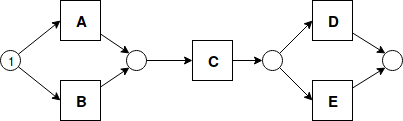
\includegraphics[width=\linewidth]{figures/algorithm/LT_Seq_01_Original.png}
	\label{fig:seq-2-original}
	\caption{One Petri net with two two xor blocks}
\end{figure}
\begin{enumerate}
	\item $LT=\{ A\rightsquigarrow D, A\rightsquigarrow E, B\rightsquigarrow D, B\rightsquigarrow D\}$. \\
	$LT_S = \{A,B\}, LT_T=\{D,E\}, \vert LT \vert = \vert XORB_S \vert * \vert XORB_T \vert  $, which means long-term dependency has all combinations of source and target xor branches. 
	\item $LT=\{ A\rightsquigarrow D, A\rightsquigarrow E, B\rightsquigarrow E\}. $\\
	$LT_S = \{A,B\}, LT_T=\{D,E\}$
	$LT_S = XORB_S $ and $LT_T = XORB_T, \vert LT \vert < \vert XORB_S \vert * \vert XORB_T \vert $. it doesn't cover all combinations. But for one xor branch $X \in XORB_S, LT_T(X)= XORB_T$, it has all the full long-term dependency with $XORB_T$. 
	\item $LT=\{ A\rightsquigarrow D, B\rightsquigarrow E\}. $\\
	$LT_S = \{A,B\}, LT_T=\{D,E\}$
	$LT_S = XORB_S $ and $LT_T = XORB_T, \vert LT \vert < \vert XORB_S \vert * \vert XORB_T \vert $. For all xor branch $X \in XORB_S, LT_T(X) \subsetneq XORB_T$, none of xor branch X has long-term dependency with $XORB_T$.
	\item $LT=\{ A\rightsquigarrow D, B\rightsquigarrow D\}.$ \\
	$LT_S = XORB_S ,  LT_T \subsetneq XORB_T$. There exists at least one xor branch $Y \in XORB_T$ which has no long-term dependency on it.
	\item $LT=\{ A\rightsquigarrow D, A\rightsquigarrow E\}.$ \\
	$LT_S \subsetneq XORB_S ,  LT_T = XORB_T$.
	There exists at least one xor branch in source $X \in XORB_S$ which has no long-term dependency on it.
	\item $LT=\{ A\rightsquigarrow E\}. $\\
	$LT_S \subsetneq XORB_S ,  LT_T \subsetneq XORB_T$.
	There exists at least one xor branch in source $X \in XORB_S$  and one xor target xor branch which has no long-term dependency on it.
	\item $ \emptyset$ . There is no long-term dependency on this set. 
\end{enumerate}
In the following, we propose a method to express long-term dependency on Petri net. 
%% should we write down here to prove the correctness of available situations, or we need to wait??
\subsection{Way to express long-term dependency}
Adding places to Petri net can limit the behavior\cite{bergenthum2007process}, since its output transitions demand a token from it to fire themselves. When there is no token at this place, the transitions are enabled. By injecting extra places on Petri net, it can block negative behaviors which are not expected in the aspect of business performance. 

Long-term dependency limits the available choices to fire transitions after the previous xor branch executes. So to express long-term dependency, our basic idea is to add places to the Petri net model. What's more, because one xor branch can be as a source to multiple long-term dependencies and one xor branch can be as a target to multiple long-term dependencies, silent transitions are also needed to address a long-term dependency explicitly. 


Given arbitrary two xor blocks, $S=\{X_1,X2,...X_m\}$ and $T=\{Y_1,Y_2,...Yn\}$ with long-term dependency $LT=\{X_i \rightsquigarrow Y_j \vert 1 \leq i \leq m, 1 \leq j \leq n \}$, we add places after the source xor branches,  $P_S=\{p_{X_i} \vert X_i \in LT_{S} \}$, and places before target xor branches,$P_T=\{p_{Y_j} \vert Y_i \in LT_{T} \}$. For each long-term dependency $X_{i} \rightsquigarrow Y_{j}$ in LT, there is silent transition t with $p_{X_i} \rightarrow t \rightarrow p_{Y_{j}}$. The steps to add silent transitions and places according to the long-term dependency are listed in algorithm \ref{alg: Adding method}.

% An algorithm is given to show how to add the long-term dependency
\begin{algorithm}[!ht]
	\SetAlgoLined
	$XORB_Y$ is dependent on $XORB_X$\;
	\If{$XORB_X$ is leaf node}{
		One place is added after this leaf node \;
	}
	\If{$XORB_X$ is Seq}{
		Add a place after  the end node of this branch\;
		The node points to the new place\;
	}
	\If{$XORB_X$ is And}{
		Create a place after the end node of every children branch in this And xor branch \; 
		Combine all the places by a silent transition after those places \;
		Create a new place directly after silent transition to represent the And xor branch \;
	}
	
	\If{$XORB_Y$ is leaf node}{
		One place is added before this leaf node \;
	}\If{$XORB_Y$ is Seq}{
		Add a place before  the end node of this branch\;
		The new place points to this end node\;
	}\If{$XORB_Y$ is And}{
		Create a place before the end node of every children branch in this And xor branch \; 
		Combine all the places by a silent transition before those places \;
		Create a new place directly before silent transition to represent the And xor branch \;
	}
	Connect the places which represent the $XORB_X$ and $XORB_Y$ by creating a silent transition.
	\caption{Add long-term dependency between pure xor branch}
	\label{alg: Adding method}
\end{algorithm}
\begin{figure}
	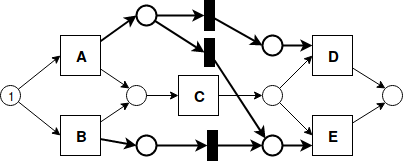
\includegraphics[width=\textwidth]{figures/algorithm/LT_Seq_01_Silent_01.png}
	\label{fig:add-algorithm-example}
	\caption{Model with long-term dependency $LT=\{ A\rightsquigarrow D, A\rightsquigarrow E, B\rightsquigarrow E\}. $ }
\end{figure}
One simple example is given in the Figure \ref{fig:add-algorithm-example} to explain this algorithm. Given the long-term dependencies $LT=\{ A\rightsquigarrow D, A\rightsquigarrow E, B\rightsquigarrow E\}$, two extra places are added respectively after A and B; Next, two places before D and E are created to express that the xor branches are involved with long-term dependency. At end, for each long-term dependency, a silent transition is generated to connect the extra places after the source xor branch to the place before target place. 

\subsection{Soundness Analysis}
% this section is used to select the sound situations. 
% next time I can go to library at Tuesday with the laptop and study there..
Following algorithm \ref{alg: Adding method} by adding silent transitions and places to express long-term dependency, the model soundness can be violated. In the following section, we discuss the soundness in different situations. 

Given a Petri net with long-term dependency $LT=\{X_i \rightsquigarrow Y_j \vert 1 \leq i \leq m, 1 \leq j \leq n \}$ on two xor blocks $S=\{X_1,X2,...X_m\}$ and $T=\{Y_1,Y_2,...Yn\}$, following the Algorithm \ref{alg: Adding method}, $P_S=\{p_{X_i} \vert X_i \in LT_{S} \}$ , $P_T=\{p_{Y_j} \vert Y_i \in LT_{T} \}$, and silent transitions $ E = \{\epsilon \vert p_{X_i} \rightarrow \epsilon
 \rightarrow p_{Y_{j}} \}$ are added. The Petri net is sound if and only if (1)the soundness outside xor blocks with long-term dependency is not violated; and  (2) soundness between xor blocks is kept. In the following, we check the model soundness with long-term dependency after applying Algorithm \ref{alg: Adding method}.
\subsubsection{(1) Soundness outside xor blocks}
\emph{Proof:} he added silent transitions and places do not violate the execution outside of the xor blocks, because the extra tokens that are generated due to long-term dependency are constrained in the xor blocks, and it doesn't affect the token flows outside. As we know, the original model is sound. So the soundness outside xor blocks is not violated.
\subsubsection{(2) Soundness inside xor blocks}
For all xor branches in S, only one branch can be fired. Without loss of generality, $X_i$ is assumed to be enabled. After firing $X_i$, the marking distribution on the extra places are  
\[ M(p_{X_i}) = 1; \quad 
\forall p_{X_i\prime} \in P_S, i\prime \neq i, M(p_{X_i\prime})=0 \]
%% here we need to divide them into different situations...
If $ LT_S = S, LT_T=T$, adding the long-term dependency in this situation doesn't violate the model soundness, we prove it in the following part.\\
%the following conditions are checked. 
\begin{itemize}
	\item safeness. Places cannot hold multiple tokens at the same time.\\
	For all extra places $p_{X_i}$ and $p_{Y_j}$, 
	\[\forall p_{X_i} \in P_S, \sum M(p_{X_i})=1\]
	Because $ LT_S = S, X_i \in S$, so $X_i \in LT_S$, there exists one $Y_j$ with $X_i \rightarrow Y_j$ and one $\epsilon, p_{X_i} \rightarrow \epsilon
	\rightarrow p_{Y_{j}} $.  After firing $X_i$, the transition $\epsilon$ becomes enable. After executing $\epsilon$, the marking distribution turns to 
	\[ M(p_{Y_j}) = 1;\quad 
	\forall p_{Y_j\prime} \in P_T, j\prime \neq j,  M(p_{Y_i})=0 \]
	So whenever the marking distribution in the extra places are
	\[\sum M(p_{X_i}) \leq 1,  \sum M(p_{Y_j}) \leq 1 \] 
	\item proper completion. If the sink place is marked, all other places are empty. \\
	After firing $Y_j$, all the extra places hold no token. So it does not violate the proper completion.
	\item option to complete.  It is always possible to reach the final marking just for the sink place. \\
	There is always one $Y_j$ enabled after firing $X_i$ to continue the subsequent execution.
	\item no dead part. For any transition there is a path from source to sink place through it. \\
	Because all $Y_j \in T$ are also in $LT_T$, there exists at least one $X_i\in S$ with long-term dependency with $Y_j$. After $X_i$ is fired, one token is generated on the extra place $p_{X_i}$ and can be consumed by silent transition $\epsilon$ in  $p_{X_i} \rightarrow \epsilon \rightarrow p_{Y_{j}}$ to produce a token in $p_{Y_j}$, which enables xor branch $Y_j$ and leaves no dead part.
\end{itemize}
Else, in other situation, the model becomes unsound. \\
\indent If $LT_S \neq S,or\quad LT_T \neq \emptyset$, there exists one xor branch $X_i$ with $X_i \notin LT_S$. When $X_i$ is fired, it generates one token at place $p_{X_i}$, this token cannot be consumed by any $Y_j$. So it violates the proper completion. \\  
\indent If $LT_T \neq T$, there exists one $Y_j \notin LT_T, \nexists X_i, X_i \rightsquigarrow Y_j$, so with two input places but $Token(p_{Y_j})=0$,  $Y_j$ becomes the dead part, which violates the soundness again. \\

As a conclusion, to keep Petri net with long-term dependency sound, only situation $ LT_S = S, LT_T=T$ is considered. However, when the long-term dependency is full connected where each combination of xor branches from source and target xor block has long-term dependency, namely xor branches can be chosen freely, we don't add any places and silent transitions on the model. 
\section{Reduce Silent Transitions}
%% We reduce the silent transition when there is no 
Our method to represent long-term dependency can introduce redundant silent transitions and places, which complicates the model. So, we post process the Petri net with long-term dependency to delete redundant silent transitions and places.
% ; on the other hand, it causes the model unsound where the extra silent transitions suspend the execution and therefore violates the soundness condition of proper completion.
\begin{proposition}
	Given a silent transition $\epsilon$ in Petri net with one input place $P_{in}$ and one output place $P_{out}$, if $\vert Outedges({P_{in}) }\vert \geq 2 \quad and \quad \vert Inedges(P_{out}) \vert \geq 2 $, the silent transitions can not be deleted. Else, the silent transitions is able to delete, meanwhile the $P_{in}$ and $P_{out}$ can be merged into one place. This reduction does not violate the soundness and does not change the model behavior.
\end{proposition}
\begin{proof}[Soundness Proof]
	If a silent transition t is able to delete, then
	\[\vert Outedges({P_{in}) }\vert \leq 1	\quad (1) \quad or, \]
	\[\vert Inedges({P_{out}) }\vert \leq 1\quad (2).\]
	When in case (1), $P_{in}$ contains a token that is always passed to $P_{out}$ by silent transitions t. After deleting the silent transition, the token is generated directly on $P_{out}$. Since t is silent transition, it won't affect the model behavior. \\ 
	when in case (2), $P_{out}$ contains a token that is always passed from $P_{in}$ by silent transitions t. After deleting the silent transition, the token is remained on $P_{in}$, which enables the later execution after the original $P_{out}$. Since t is silent transition, it won't affect the model behavior. \\
	In other cases, $Outedges({P_{in}) }\vert \geq 2 \quad and \quad \vert Inedges(P_{out}) \vert \geq 2$, which means that the source xor branch with output place $P_{in}$ has at lest two long-term dependencies; the target xor branch with input place $P_{out}$ has at least two long-term dependencies. If we delete this silent transitions, the long-term dependencies are mixed together which allows more unexpected behaviors. Therefore, silent transition in this situation is necessary to hold long-term dependency.
\end{proof}
%% here we need to prove this proposition
One example is given in the following graph. $M_{lt}$ in Figure \ref{fig:with-lt} has long-term dependency expressed in the silent transitions and places. The silent transition for $S2 \rightsquigarrow B1 $ and silent transition for $B1 \rightsquigarrow T2$ belongs to the case (1). So they are kept in the model, while the other silent transitions are deleted. After reducing the redundant silent transitions, the model becomes $M_r$ shown in Figure \ref{fig:reduced-lt}. Those two models have the same behavior, yet the reduced model is simpler.
\begin{figure}[!h]
	\centering
	\begin{subfigure}[a]{\textwidth}
		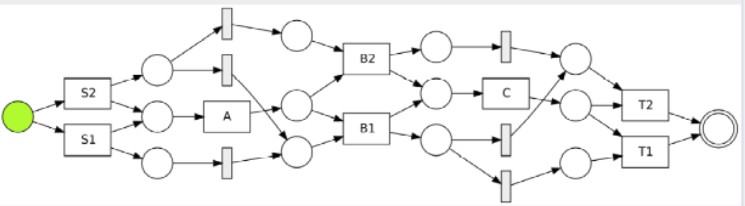
\includegraphics[width=\textwidth]{figures/algorithm/dfg-IM-pn-with-lt.png}
		\label{fig:with-lt}
		\caption{A Petri net $M_{lt}$ with redundant silent transitions}
	\end{subfigure}
	\hfill
	\begin{subfigure}[b]{\textwidth}
		\centering
		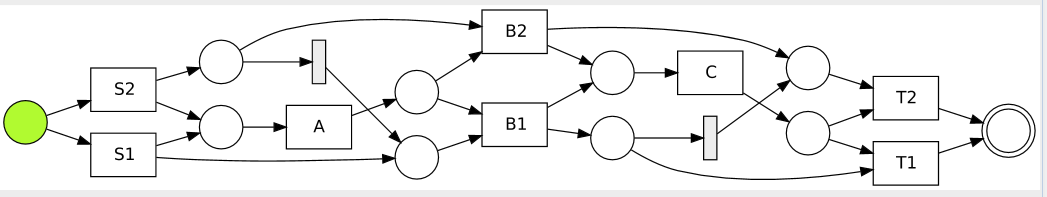
\includegraphics[width=\linewidth]{figures/algorithm/dfg-IM-pn-with-lt-reduced.png}
		\label{fig:reduced-lt}
		\caption{Petri net $M_r$ with reduced silent transitions}
	\end{subfigure}
\end{figure}

